%!TEX root = ../report.tex

% 
% Related work
% 

\section{Related Work}

%TODO: Rewrite Related Work Intro

%The following section starts to present the use of refactoring tools and an overview of static refactoring tools. 
%Then it presents the refactoring tools for the dynamic languages such as, Scheme, JavaScript, Smalltalk, Python and Racket.
%Finally it has a conclusion about the related work.


\subsection{Formal Pattern Language for Refactoring of Lisp Programs}
%prof paper
In this paper \cite{leitdo2002formal} it is proposed a pattern language refactoring tool that works well on lisp-like languages. 

The pattern is composed by transformations that are described in a simple syntax and even that the pattern is composed by operations of simple syntax they are composable, which makes it easier for the programmer to extend the refactoring tool, and there is no impediment to create complex transformations.

The tool also can induce transformation rules based on manual examples given by the programmer and then if needed the programmer can easily extend those rules.

This tool is simple because it is focused on syntax transformations of the program. Meaning that it does not need semantic information such as bindings relations needed for transformations, making it a simpler tool.


\subsection{HaRe}

The HaRe system is a refactoring tool for Haskell that integrates with Emacs and Vim.
This tool was made for the working programmers instead of being a prof of concept prototype and it is implemented in Haskell.

The HaRe system also allows the users to design their own refacatorings using the HaRe API.

\subsubsection{Representation}
\hfill \break

The HaRe \cite{thompson2005refactoring} system uses an AST of the program to be refactored in order to reason about the transformations to do.
The system also have a token stream in order to preserve the comments and the program layout by keep information about the source code location and the comments of all tokens.

\subsubsection{Stages of Refactoring}
\hfill \break

{\bf Information gathering and condition checking:} The Refactoring will only be performed if it preserves the semantics of the program.
It is needed some information, such as a set of identifiers of the scope, that information is gathered trough transversing the AST.

{\bf Transformation:} After the conditions are verified, it is possible to apply the refactoring operation, which is a transformation of the AST.

{\bf Program rendering:} After the refactoring operation the source code of the new program needs to be generated, keeping the original program layout as much as possible.

%insert pic?
\begin{figure}[h!]
  \centering
  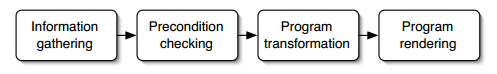
\includegraphics[width=0.75\textwidth]{img/HaReStagesOfRefactoring.png}
  \caption{Stages of Refactoring}
  \label{fig:HaReStages}
\end{figure}
%add structural refactorings, module-aware? 

\subsubsection{Refactorings Available} %review and change title
\hfill \break

Initially the HaRe system only had structural refactorings. 
Structural refactorings care about the objects defined in the program, the name and the scope of those objects. Examples of this are: Delete, Duplicate, Rename, Promote, Demote, etc \ldots
Then it was added module awareness to those refactorings. 
Module awareness is important because in Haskell it is possible to import definitions from other modules.
With module awareness it was possible to add new refactorings to the module like Clean the imported list, move a definition to another module or add and remove items of the export list.

\subsection{Scheme}
%Griswold
%Characteristics Dynamic language, Simple refactoring operations, Only One language, AST?, PDG?, Easy to create new operations?

Griswold \cite{griswold1991program} proved that meaning-preserving restructuring can substantively reduce the maintenance cost of a system.
A prototype was created to prove the concept, by creating restructuring operations for the Scheme programming language implemented in Common Lisp.
The prototype was developed for Scheme because of it's imperative features, simple syntax and it was available a (program dependence graph) PDG for Scheme implemented in Common Lisp
The prototype had simple restructuring operations to prove the concept, such as: moving an expression, renaming a variable, abstracting an expression, extracting a function, scope-wide function replacement, adding a reference indirection and adding looping to list references.

\subsubsection{Tool aided vs Manual Restructuring}
Griswold starts comparing automated restructuring with manual restructuring. 
To do that Griswold creates an experience.
It was given an initial program and a description of four transformations goals to six subjects.%An initial program and a description of the four goals of the transformations to be made was presented to 6 subjects. 

Although it was a experience with a small number of subjects, Griswold took several conclusions on how people manually restructure programs.
People use the copy/paste and the cut/paste paradigm to do the transformations. 
This means that they copy or cut the code and then paste it in the desired location.
Although the Cut/Paste paradigm is more dangerous because it is a destructive operation. 
This means if the user makes any error it is more difficult to correct it because it is a destructive operation.

Griswold also conclude that people make mistakes even with small and simple programs. 
And the cost of correcting mistakes is higher than the time to do the restructuring itself. 
And it also conclude that manual restructuring is haphazard. 
Meaning that the transformations were done in almost a random way when compared to the computer-assisted process.


\subsubsection{Architecture}



In order to be able to correctly implement these operations it was used contours and a PDG (program dependence graph).

The main program representation is the contours. 
Contours are an abstraction of the essential semantic properties that the AST (abstract syntax tree) represents in an efficient and complete form.

Whereas the PDG explicitly represents the key relationship of dependence between the operations in the program. 
The PDG is used because simple graph algorithms can extract this information and it has been a popular program representation for aiding program parallelization, optimization and version merging.
This features combined with the right semantic support make the PDGs a good foundation for preserving meaning during restructuring.
With these structures it is possible to combine them and have a single formalism to reason effectively about flow dependencies and scope structure.

%It is possible to have this representation because it have access to everything like a compiler does, and it tries to used work done, such as using a library for the PDG. Using DrRacket the semantic part is covered by the arrows created which helps having the semantic logic between things.

